\section{Quantity 1: Viability}

\intuitbox{The pupil is a fixed-size circular opening. A hole only contributes light if
its own circle overlaps the pupil's circle. If the nearest hole to the
optical axis is too far away, or too small, to reach the pupil at all, the
wearer looking straight ahead sees nothing through this design --- a
blackout. This is the single defect that has broken this project's winner
list twice.
}
\subsection{The Check}
A hole at distance $d$ from the pupil center overlaps the pupil if
\begin{equation}
d - R_h < R_p
\end{equation}
where $R_h$ is the hole radius and $R_p$ is the pupil radius. If this fails
for every hole in the design, the design is a blackout.

\subsection{The Full Overlap Area (when it does overlap)}
\begin{equation}
A = R_p^2\cos^{-1}\!\left(\frac{d^2{+}R_p^2{-}R_h^2}{2dR_p}\right)
  + R_h^2\cos^{-1}\!\left(\frac{d^2{+}R_h^2{-}R_p^2}{2dR_h}\right)
  - \tfrac12\sqrt{(-d{+}R_p{+}R_h)(d{+}R_p{-}R_h)(d{+}R_h{-}R_p)(d{+}R_p{+}R_h)}
\end{equation}

\begin{figure}[h]
\centering
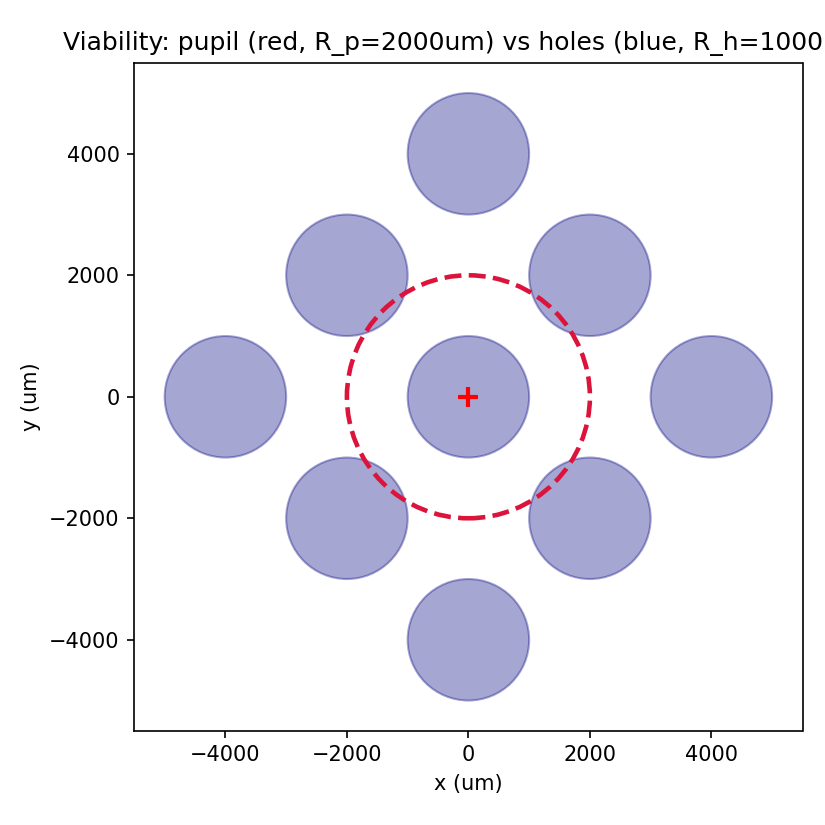
\includegraphics[width=0.55\textwidth]{verification_pdf_figs/fig_viability.png}
\caption{Pupil (red dashed circle, $R_p=2000\mu$m) against every hole (blue,
$R_h=1000\mu$m) in the worked example of Sec.~5. The central hole sits
exactly at the pupil center, so this design is trivially viable.}
\end{figure}

\checkbox{Find the hole nearest the pupil center in the design's own coordinate list.
Compute $d$ as the straight-line distance from that hole to the pupil center
(at straight-ahead gaze, the pupil center is the origin). Check the one-line
inequality above --- no need for the full overlap-area formula unless you
also want the exact transmitted area.
}
\newpage
